% =====================================================================
% Fundamentos de Sistemas Electrónicos Analógicos - BJT NPN
% Compilar: pdflatex clase_3_bjt_npn.tex  (2 pasadas)
% =====================================================================
\documentclass[aspectratio=169]{beamer}

\usepackage[utf8]{inputenc}
\usepackage[T1]{fontenc}
\usepackage{lmodern}
\usepackage[spanish,es-tabla]{babel}
\usepackage{amsmath,amssymb}
\usepackage{siunitx}
\usepackage{booktabs}
\usepackage{array}
\usepackage{microtype}
\usepackage{circuitikz}
\usepackage{pgfplots}
\usepgfplotslibrary{groupplots}
\pgfplotsset{compat=1.18}

\definecolor{navy}{RGB}{23,54,93}
\definecolor{navysoft}{RGB}{72,101,140}
\definecolor{gold}{RGB}{179,142,62}
\definecolor{ink}{RGB}{44,51,58}
\definecolor{soft}{RGB}{244,241,234}

\usetheme{default}
\setbeamertemplate{navigation symbols}{}
\setbeamertemplate{footline}[frame number]
\setbeamercolor{structure}{fg=navy}
\setbeamercolor{frametitle}{fg=white,bg=navy}
\setbeamercolor{title}{fg=navy}
\setbeamercolor{subtitle}{fg=navysoft}
\setbeamercolor{itemize item}{fg=gold}
\setbeamercolor{itemize subitem}{fg=gold}
\setbeamercolor{block title}{fg=white,bg=navy}
\setbeamercolor{block body}{bg=soft}
\setbeamercolor{example text}{fg=navy}
\setbeamertemplate{itemize item}{\scriptsize\raise1.25pt\hbox{\donotcoloroutermaths$\bullet$}}
\setbeamertemplate{itemize subitem}{\scriptsize\raise1.25pt\hbox{\donotcoloroutermaths$\circ$}}
\setbeamerfont{frametitle}{size=\large,series=\bfseries}

\title[BJT NPN]{Transistor de Unión Bipolar (BJT) tipo NPN}
\subtitle{Clase de teoría · Fundamentos de Sistemas Electrónicos Analógicos}
\institute{Licenciatura en Ingeniería Aeroespacial · UNAM}
\date{Semestre 2027-1}

\begin{document}

% ---------------------------------------------------------------------
\begin{frame}[plain]
  \titlepage
\end{frame}

% ---------------------------------------------------------------------
\begin{frame}{Objetivos}
  \begin{itemize}
    \item Relacionar la estructura N-P-N con el símbolo y el modelo equivalente del transistor.
    \item Seguir la respuesta del circuito al barrer la fuente de entrada entre
      $-5$ y $10\,\mathrm{V}$.
    \item Identificar, en orden, las regiones de \textbf{corte}, \textbf{activa} y
      \textbf{saturación}.
    \item Calcular $I_B$, $I_C$ y $V_{CE}$ en cada región.
    \item Determinar la corriente máxima de colector y la entrada que inicia la saturación.
    \item Relacionar el análisis con aplicaciones y restricciones aeroespaciales.
  \end{itemize}
\end{frame}

% ---------------------------------------------------------------------
\begin{frame}{1 · De la estructura N-P-N al símbolo}
  \begin{columns}[T]
    \begin{column}{0.31\textwidth}
      \centering
      \textbf{Estructura física}\\[5pt]
      \begin{tikzpicture}[scale=0.72]
        \draw[fill=blue!25] (0,0) rectangle (2.5,0.9);
        \draw[fill=red!20]  (0,0.9) rectangle (2.5,1.7);
        \draw[fill=blue!25] (0,1.7) rectangle (2.5,2.6);
        \draw (1.25,0) -- (1.25,-0.55) node[below] {Emisor};
        \draw (0,1.3) -- (-0.55,1.3) node[left] {Base};
        \draw (1.25,2.6) -- (1.25,3.15) node[above] {Colector};
        \node at (1.25,2.15) {N};
        \node at (1.25,1.3) {P};
        \node at (1.25,0.45) {N};
      \end{tikzpicture}
      \par\scriptsize La base es delgada; el emisor inyecta portadores y el colector los recoge.
    \end{column}
    \begin{column}{0.35\textwidth}
      \centering
      \textbf{Dos uniones PN}\\[8pt]
      \begin{circuitikz}[scale=0.72, transform shape]
        \draw (0,0) node[left] {B} to[short, o-] (1.15,0);
        \draw (1.15,0) -- (1.15,1.35) to[D] (3.0,1.35) node[right] {C};
        \draw (1.15,0) -- (1.15,-1.35) to[D] (3.0,-1.35) node[right] {E};
      \end{circuitikz}
      \par\scriptsize La base P es el ánodo común de las uniones base-colector y base-emisor.
    \end{column}
    \begin{column}{0.27\textwidth}
      \centering
      \textbf{Símbolo NPN}\\[12pt]
      \begin{circuitikz}[scale=1.35]
        \node[npn] (Q) at (0,0) {};
        \node[left] at (Q.B) {$B$};
        \node[above] at (Q.C) {$C$};
        \node[below] at (Q.E) {$E$};
      \end{circuitikz}
      \vspace{10pt}
      \par\scriptsize Regla visual: en un NPN la flecha del emisor apunta hacia afuera (``no pincha'').
    \end{column}
  \end{columns}
  \vfill
  \begin{block}{Alcance del dibujo de uniones}
    Las dos uniones describen la estructura, pero dos diodos aislados no reproducen
    la acción transistor; en región activa se necesita el modelo con fuente dependiente.
  \end{block}
\end{frame}

% ---------------------------------------------------------------------
\begin{frame}{2 · Una corriente pequeña controla otra mayor}
  \begin{columns}[T]
    \begin{column}{0.48\textwidth}
      \centering
      \begin{circuitikz}[american voltages, scale=0.82]
        \draw (0,2.7) node[left] {B} to[short, o-] (0.55,2.7)
          to[D] (3.0,2.7) -- (3.0,0) node[ground] {} node[right] {E};
        \draw (5.2,4.0) node[above] {C} to[short, o-] (5.2,3.35)
          to[cI] (5.2,0) -- (3.0,0);
        \draw[->, thick, navy] (0.65,3.25) -- (1.65,3.25)
          node[midway,above] {$I_B$};
        \draw[->, thick, navy] (5.8,3.3) -- (5.8,2.2)
          node[midway,right] {$I_C$};
        \node[right] at (5.7,1.65) {$\beta I_B$};
        \node[below] at (1.75,2.55) {$V_{BE}\approx0.7\,\mathrm{V}$};
      \end{circuitikz}
    \end{column}
    \begin{column}{0.48\textwidth}
      \textbf{En región activa}
      \[
        I_C=\beta I_B=h_{FE}I_B,
        \qquad I_E=I_B+I_C.
      \]
      \begin{itemize}
        \item $I_B$ e $I_C$ entran al dispositivo; $I_E$ sale.
        \item $\beta$ es la ganancia estática de corriente del modelo.
        \item Si $I_B=0$, la fuente dependiente vale cero y también $I_C=0$.
        \item En saturación, la red externa impide mantener $I_C=\beta I_B$.
      \end{itemize}
    \end{column}
  \end{columns}
\end{frame}

% ---------------------------------------------------------------------
\begin{frame}{3 · La analogía del grifo anticipa las tres regiones}
  \begin{columns}[T]
    \begin{column}{0.55\textwidth}
      \begin{enumerate}
        \item \textbf{Corte:} el grifo está cerrado; no hay flujo, por lo que $I_C=0$.
        \item \textbf{Activa:} al abrir la llave, el flujo aumenta de forma aproximadamente proporcional a $I_B$.
        \item \textbf{Saturación:} el sistema entrega su caudal máximo; abrir más la llave ya no aumenta $I_C$.
      \end{enumerate}
      \begin{block}{Qué representa cada elemento}
        Llave $\leftrightarrow I_B$; caudal $\leftrightarrow I_C$; límite hidráulico
        $\leftrightarrow$ fuente y resistencia de colector.
      \end{block}
    \end{column}
    \begin{column}{0.41\textwidth}
      \centering
      \begin{tikzpicture}[scale=0.88]
        \draw[very thick, fill=gray!22] (0,2.0) -- (3.1,2.0) -- (3.1,1.15)
          -- (2.35,1.15) -- (2.35,1.45) -- (0,1.45) -- cycle;
        \draw[very thick] (1.75,2.0) -- (1.75,2.75);
        \draw[very thick] (1.15,2.75) -- (2.35,2.75);
        \draw[->, very thick, navy] (1.75,3.55) -- (1.75,2.95)
          node[above,yshift=5pt] {Llave: $I_B$};
        \draw[very thick, navy] (2.72,1.1) .. controls (2.72,0.55) and (3.55,0.55) .. (3.55,-0.05);
        \draw[->, very thick, navy] (3.55,-0.05) -- (3.55,-0.75)
          node[below] {Caudal: $I_C$};
        \node at (1.25,1.72) {Grifo};
      \end{tikzpicture}
      \vspace{8pt}
      \par\small La analogía explica el comportamiento; las mallas siguientes fijan los valores numéricos.
    \end{column}
  \end{columns}
\end{frame}

% ---------------------------------------------------------------------
\begin{frame}{4 · Circuito y barrido de entrada}
  \begin{columns}[T]
    \begin{column}{0.55\textwidth}
      \begin{center}
      \begin{circuitikz}[american voltages, scale=0.72, transform shape]
        \node[npn] (Q) at (3.6,1.45) {};
        \draw (0,2.35) to[V, l_={$V_S$}] (0,0);
        \draw (0,2.35) to[R, l={$R_B=50\,\mathrm{k}\Omega$}] (Q.B);
        \node[navy] at (2.45,1.05) {$I_B\;\longrightarrow$};
        \draw (Q.E) -- (3.6,0) -- (0,0);
        \draw (6.5,3.35) to[V, l={$V_{CC}=15\,\mathrm{V}$}] (6.5,0) -- (3.6,0);
        \draw (6.5,3.35) -- (4.6,3.35)
          to[R, l={$R_C=1.5\,\mathrm{k}\Omega$}] (4.6,1.75) -- (Q.C);
        \draw[->, navy, thick] (4.15,3.15) -- (4.15,2.45)
          node[midway,right] {$I_C$};
        \node[ground] at (3.6,0) {};
        \draw[->, navy, thick] (4.35,1.95) -- (4.35,0.75)
          node[midway,right] {$V_{CE}$};
      \end{circuitikz}
      \end{center}
    \end{column}
    \begin{column}{0.41\textwidth}
      \textbf{Entrada variable}
      \[
        -5\,\mathrm{V}\leq V_S\leq 10\,\mathrm{V}
      \]
      \textbf{Datos del modelo}
      \[
        \beta=100,\qquad V_{BE}=0.7\,\mathrm{V}
      \]
      \textbf{Seguiremos}
      \[
        I_B,\qquad I_C,\qquad V_{CE}
      \]
    \end{column}
  \end{columns}
\end{frame}

% ---------------------------------------------------------------------
\begin{frame}{5 · Corte: la unión base-emisor no conduce}
  \begin{columns}[T]
    \begin{column}{0.48\textwidth}
      Si $V_S<0.7\,\mathrm{V}$, la unión base-emisor no alcanza su tensión directa:
      \[
        I_B=0,\qquad I_C=0.
      \]
      El transistor se comporta como un \textbf{circuito abierto} entre colector y emisor.
    \end{column}
    \begin{column}{0.48\textwidth}
      \begin{center}
      \begin{circuitikz}[american voltages, scale=0.74]
        \draw (0,3) to[V, l_={$15\,\mathrm{V}$}] (0,0) -- (4.5,0);
        \draw (0,3) to[R, l={$R_C$}] (3,3)
          to[ospst, l={$Q$}, i>^={$I_C=0$}] (3,0);
        \node[ground] at (4.5,0) {};
        \draw[<->, navy, thick] (4,2.85) -- (4,0.15)
          node[midway,right] {$V_{CE}=15\,\mathrm{V}$};
      \end{circuitikz}
      \end{center}
    \end{column}
  \end{columns}
  \begin{block}{Resultado en corte}
    No existe caída en $R_C$; por ello toda la alimentación aparece como $V_{CE}$.
  \end{block}
\end{frame}

% ---------------------------------------------------------------------
\begin{frame}{6 · Al superar 0.7 V comienza la región activa}
  Para $V_S>0.7\,\mathrm{V}$ aparece corriente de base:
  \[
    I_B=\frac{V_S-V_{BE}}{R_B}
       =\frac{V_S-0.7}{50\,\mathrm{k}\Omega}.
  \]
  Mientras el transistor permanezca en región activa:
  \[
    I_C=\beta I_B,
    \qquad
    V_{CE}=V_{CC}-I_C R_C.
  \]
  \begin{block}{Evolución al aumentar $V_S$}
    $I_B$ aumenta $\Rightarrow$ $I_C$ aumenta $\Rightarrow$
    la caída $I_C R_C$ aumenta $\Rightarrow$ $V_{CE}$ disminuye.
  \end{block}
\end{frame}

% ---------------------------------------------------------------------
\begin{frame}{7 · Las dos mallas en región activa}
  \begin{center}
  \begin{circuitikz}[american voltages, scale=0.84]
    \draw (0,2.8) to[V, l_={$V_S$}] (0,0);
    \draw (0,2.8) to[R, l={$R_B$}, i>^=$I_B$] (3.2,2.8)
      to[D] (3.2,0) -- (0,0);
    \node[left, align=right] at (3.05,1.35) {$V_{BE}\approx{}$\\$0.7\,\mathrm{V}$};
    \draw (8,3.4) to[V, l={$V_{CC}$}] (8,0) -- (5.2,0);
    \draw (8,3.4) to[R, l={$R_C$}, i>^=$I_C$] (5.2,3.4)
      to[cI] (5.2,0);
    \node[right] at (5.65,1.7) {$\beta I_B$};
    \node[ground] at (4.2,0) {};
  \end{circuitikz}
  \end{center}
  \begin{itemize}
    \item La rama de base se aproxima por un diodo de $0.7\,\mathrm{V}$.
    \item La rama de colector se representa con una fuente controlada de valor $\beta I_B$.
    \item Este modelo sólo es válido mientras la red permita que $I_C=\beta I_B$.
  \end{itemize}
\end{frame}

% ---------------------------------------------------------------------
\begin{frame}{8 · La red fija una corriente máxima de colector}
  La mayor corriente aparece cuando $V_{CE}$ llega a su valor mínimo. Para seguir
  el modelo simplificado usamos $V_{CE,\min}=0$:
  \[
    I_{C,\max}
      =\frac{V_{CC}-V_{CE,\min}}{R_C}
      =\frac{15-0}{1.5\,\mathrm{k}\Omega}
      =\SI{10}{\milli\ampere}.
  \]
  \begin{block}{Interpretación}
    Cuando $\beta I_B$ intenta superar $\SI{10}{\milli\ampere}$, la resistencia
    $R_C$ y la fuente de $15\,\mathrm{V}$ impiden que $I_C$ continúe aumentando:
    el transistor entra en \textbf{saturación}.
  \end{block}
  {\small En un transistor real suele emplearse $V_{CE,sat}\approx0.2$--$0.3\,\mathrm{V}$; el procedimiento es el mismo.}
\end{frame}

% ---------------------------------------------------------------------
\begin{frame}{9 · Corriente de base en el límite de saturación}
  Justo en la frontera entre región activa y saturación todavía podemos usar
  $I_C=\beta I_B$:
  \[
    I_{B,sat}
      =\frac{I_{C,\max}}{\beta}
      =\frac{10\,\mathrm{mA}}{100}
      =\SI{0.1}{\milli\ampere}.
  \]
  \begin{block}{Punto crítico}
    Para $I_B<0.1\,\mathrm{mA}$, $I_C=\beta I_B$.
    Para $I_B>0.1\,\mathrm{mA}$, la corriente de base puede seguir aumentando,
    pero $I_C$ queda limitada aproximadamente a $10\,\mathrm{mA}$.
  \end{block}
\end{frame}

% ---------------------------------------------------------------------
\begin{frame}{10 · La saturación comienza con $V_S=5.7$ V}
  Aplicamos KVL en la malla de base con signos coherentes:
  \[
    V_S-I_B R_B-V_{BE}=0
    \qquad\Longrightarrow\qquad
    V_S=I_B R_B+V_{BE}.
  \]
  En el límite de saturación:
  \[
    V_{S,sat}
      =(0.1\,\mathrm{mA})(50\,\mathrm{k}\Omega)+0.7\,\mathrm{V}
      =5+0.7
      =\SI{5.7}{\volt}.
  \]
  \begin{block}{Dos umbrales del barrido}
    $0.7\,\mathrm{V}$ inicia la conducción; $5.7\,\mathrm{V}$ inicia la saturación.
  \end{block}
  {\small\textbf{Control de signos:} $V_{BE}$ se suma a la caída $I_BR_B$; por ello
  el resultado coherente con KVL es $5+0.7=5.7\,\mathrm{V}$.}
\end{frame}

% ---------------------------------------------------------------------
\begin{frame}{11 · Modelo por regiones}
  \begin{table}
    \footnotesize
    \setlength{\tabcolsep}{3pt}
    \renewcommand{\arraystretch}{1.18}
    \begin{tabular}{>{\raggedright\arraybackslash}p{0.15\textwidth}
                    >{\raggedright\arraybackslash}p{0.22\textwidth}
                    >{\raggedright\arraybackslash}p{0.32\textwidth}
                    >{\raggedright\arraybackslash}p{0.22\textwidth}}
      \toprule
      Región & Intervalo de $V_S$ & Corrientes & Tensión $V_{CE}$ \\
      \midrule
      \textbf{Corte} & $V_S<0.7\,\mathrm{V}$
        & $I_B=0$, $I_C=0$
        & $V_{CE}=15\,\mathrm{V}$ \\
      \textbf{Activa} & $0.7\le V_S\le5.7\,\mathrm{V}$
        & $I_B=\dfrac{V_S-0.7}{50\,\mathrm{k}\Omega}$;\newline
          $I_C=100I_B$
        & $V_{CE}=15-I_C(1.5\,\mathrm{k}\Omega)$ \\
      \textbf{Saturación} & $V_S>5.7\,\mathrm{V}$
        & $I_B$ aumenta; $I_C\approx10\,\mathrm{mA}$
        & $V_{CE}\approx0\,\mathrm{V}$ \\
      \bottomrule
    \end{tabular}
  \end{table}
  \begin{block}{Límite del modelo}
    En saturación deja de cumplirse $I_C=\beta I_B$ porque la red externa fija el máximo.
  \end{block}
\end{frame}

% ---------------------------------------------------------------------
\begin{frame}{12 · Barrido completo respecto a $V_S$}
  \begin{center}
  \begin{tikzpicture}
    \begin{groupplot}[
      group style={group size=1 by 3, vertical sep=0.22cm, x descriptions at=edge bottom},
      width=10.8cm,
      height=1.35cm,
      scale only axis,
      xmin=-5, xmax=10,
      grid=major,
      tick label style={font=\scriptsize},
      label style={font=\scriptsize},
      every axis plot/.append style={very thick}
    ]
      \nextgroupplot[ylabel={$I_B$ (mA)}, ymin=0, ymax=0.20, ytick={0,0.1,0.2}, xticklabels={}]
        \addplot[navy, domain=-5:0.7, samples=2] {0};
        \addplot[navy, domain=0.7:10, samples=60] {(x-0.7)/50};
        \addplot[dashed, gray] coordinates {(0.7,0) (0.7,0.20)};
        \addplot[dashed, gray] coordinates {(5.7,0) (5.7,0.20)};
      \nextgroupplot[ylabel={$I_C$ (mA)}, ymin=0, ymax=11, ytick={0,5,10}, xticklabels={}]
        \addplot[gold, domain=-5:0.7, samples=2] {0};
        \addplot[gold, domain=0.7:5.7, samples=60] {2*(x-0.7)};
        \addplot[gold, domain=5.7:10, samples=2] {10};
        \addplot[dashed, gray] coordinates {(0.7,0) (0.7,11)};
        \addplot[dashed, gray] coordinates {(5.7,0) (5.7,11)};
      \nextgroupplot[xlabel={$V_S$ (V)}, ylabel={$V_{CE}$ (V)}, ymin=0, ymax=16, ytick={0,5,10,15}]
        \addplot[ink, domain=-5:0.7, samples=2] {15};
        \addplot[ink, domain=0.7:5.7, samples=60] {15-3*(x-0.7)};
        \addplot[ink, domain=5.7:10, samples=2] {0};
        \addplot[dashed, gray] coordinates {(0.7,0) (0.7,16)};
        \addplot[dashed, gray] coordinates {(5.7,0) (5.7,16)};
    \end{groupplot}
  \end{tikzpicture}
  \end{center}
  {\scriptsize Líneas verticales: inicio de conducción ($0.7\,\mathrm{V}$) e inicio de saturación ($5.7\,\mathrm{V}$).}
\end{frame}

% ---------------------------------------------------------------------
\begin{frame}{Ampliación · Encapsulados y disipación}
  \begin{columns}[T]
    \begin{column}{0.48\textwidth}
      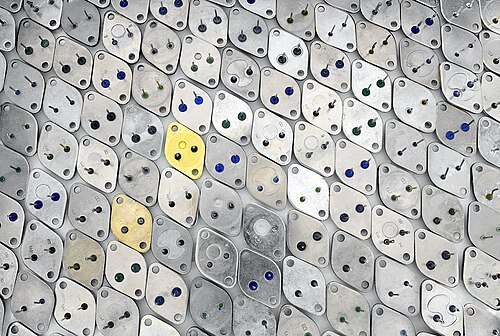
\includegraphics[height=0.38\textheight]{figs/bjt_pkg_to_3_package_botto.jpg}\\[2pt]
      \scriptsize TO-3: potencia y montaje a chasis.
    \end{column}
    \begin{column}{0.48\textwidth}
      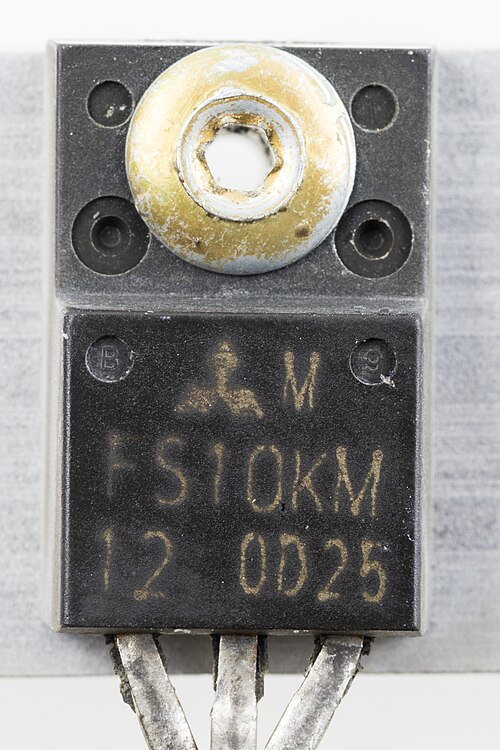
\includegraphics[height=0.38\textheight]{figs/bjt_pkg_sony_vpl_hs1___lam.jpg}\\[2pt]
      \scriptsize TO-220 sobre disipador.
    \end{column}
  \end{columns}
  \vfill
  \begin{itemize}
    \item TO-92: señal; TO-126/TO-220: potencia; TO-3: alta potencia y chasis.
    \item El encapsulado se selecciona por potencia, temperatura, montaje y ambiente.
  \end{itemize}
\end{frame}

% ---------------------------------------------------------------------
\begin{frame}{Aplicación aeroespacial}
  \begin{itemize}
    \item En región activa el BJT puede amplificar señales de sensores y telemetría.
    \item En corte y saturación funciona como interruptor para relés, calentadores y cargas auxiliares.
    \item La variación de $\beta$ y temperatura desplaza el punto de operación; un diseño robusto
      no debe depender de un único valor nominal de $\beta$.
    \item En vacío no hay convección: deben verificarse $P=V_{CE}I_C$, temperatura de unión,
      disipación por conducción/radiación y derating.
    \item El análisis por regiones permite comprobar estados seguros ante cambios de alimentación y carga.
  \end{itemize}
\end{frame}

% ---------------------------------------------------------------------
\begin{frame}{Resumen operativo}
  \begin{itemize}
    \item $V_S<0.7\,\mathrm{V}$: \textbf{corte}, $I_B=I_C=0$ y $V_{CE}=15\,\mathrm{V}$.
    \item $0.7\le V_S\le5.7\,\mathrm{V}$: \textbf{activa}, $I_C=\beta I_B$ y $V_{CE}$ disminuye.
    \item $V_S>5.7\,\mathrm{V}$: \textbf{saturación}, $I_C\approx10\,\mathrm{mA}$ y
      $V_{CE}\approx0$ en el modelo simplificado.
    \item La frontera se obtiene primero con $I_{C,\max}$, después con $I_{B,sat}$ y finalmente con KVL.
    \item Para un modelo real, sustituye $V_{CE,\min}$ por el $V_{CE,sat}$ especificado.
  \end{itemize}
\end{frame}

% ---------------------------------------------------------------------
\begin{frame}{Preguntas de verificación}
  \begin{enumerate}
    \item ¿Qué ocurre si $V_S<0.7\,\mathrm{V}$?
      \uncover<2->{\emph{($I_B=I_C=0$ y $V_{CE}=15\,\mathrm{V}$.)}}
    \item ¿Qué relaciones se usan en la región activa?
      \uncover<3->{\emph{($I_B=(V_S-0.7)/R_B$, $I_C=\beta I_B$ y $V_{CE}=V_{CC}-I_CR_C$.)}}
    \item ¿Por qué deja de crecer $I_C$ en saturación?
      \uncover<4->{\emph{(La fuente y $R_C$ limitan la corriente máxima.)}}
    \item ¿Cuánto vale $I_{C,\max}$ con $15\,\mathrm{V}$ y $1.5\,\mathrm{k}\Omega$?
      \uncover<5->{\emph{($10\,\mathrm{mA}$ en el modelo con $V_{CE,\min}=0$.)}}
    \item ¿Con qué entrada comienza la saturación?
      \uncover<6->{\emph{($I_{B,sat}=0.1\,\mathrm{mA}$ y $V_{S,sat}=5.7\,\mathrm{V}$.)}}
  \end{enumerate}
\end{frame}

\end{document}
